%% =====================================================================
%%  Resolve, Don't Remember -- IEEE conference format (IEEEtran)
%%  Build:  tectonic main.tex     (or pdflatex/bibtex/pdflatex x2)
%%  Numbers come from macros.tex and tab_*.tex, generated by
%%  paper/analysis/gen_tex.py from the raw benchmark results.
%% =====================================================================
\documentclass[conference]{IEEEtran}
\usepackage[T1]{fontenc}

\usepackage{cite}
\usepackage{amsmath,amssymb}
\usepackage{graphicx}
\usepackage{booktabs}
\usepackage{array}
\usepackage{microtype}
\usepackage{tikz}
\usetikzlibrary{arrows.meta,positioning,calc,fit,backgrounds}
\usepackage[colorlinks=true,linkcolor=blue!55!black,citecolor=blue!55!black,urlcolor=blue!55!black]{hyperref}
\graphicspath{{../figs/}}
\newcommand{\nPages}{30}
\newcommand{\nTimed}{14}
\newcommand{\nTargets}{10}
\newcommand{\nSeeds}{5}
\newcommand{\nOps}{8}
\newcommand{\nTrials}{60{,}475}
\newcommand{\nRows}{1{,}209{,}500}
\newcommand{\oursC}{72.2}
\newcommand{\oursW}{9.7}
\newcommand{\oursA}{18.1}
\newcommand{\oursCci}{67.0--76.6}
\newcommand{\oursWci}{7.5--12.3}
\newcommand{\marginC}{70.7}
\newcommand{\marginW}{5.9}
\newcommand{\marginA}{23.4}
\newcommand{\marginWci}{3.8--8.1}
\newcommand{\deltaGate}{0.05}
\newcommand{\rnC}{66.1}
\newcommand{\rnW}{21.4}
\newcommand{\textC}{57.1}
\newcommand{\textW}{32.4}
\newcommand{\chainC}{58.2}
\newcommand{\chainW}{34.2}
\newcommand{\cssC}{11.3}
\newcommand{\cssW}{6.2}
\newcommand{\cssA}{82.5}
\newcommand{\xpC}{8.5}
\newcommand{\xpW}{4.6}
\newcommand{\xpA}{86.8}
\newcommand{\strictC}{49.8}
\newcommand{\strictW}{3.0}
\newcommand{\strictA}{47.2}
\newcommand{\simC}{93.6}
\newcommand{\simW}{6.4}
\newcommand{\simA}{0.0}
\newcommand{\dCsim}{-21.5}
\newcommand{\dCsimLo}{-27.6}
\newcommand{\dCsimHi}{-16.2}
\newcommand{\dWsim}{-3.3}
\newcommand{\dWsimLo}{-5.9}
\newcommand{\dWsimHi}{-0.5}
\newcommand{\dCmsim}{-22.9}
\newcommand{\dWmsim}{0.6}
\newcommand{\simmC}{92.0}
\newcommand{\simmW}{5.0}
\newcommand{\simmA}{3.0}
\newcommand{\simmWci}{2.7--7.7}
\newcommand{\deltaSim}{0.0}
\newcommand{\dCmsimm}{21.4}
\newcommand{\dWsimmOM}{-0.9}
\newcommand{\vTwoC}{94.4}
\newcommand{\vTwoW}{5.6}
\newcommand{\vTwoA}{0.0}
\newcommand{\vTwoCci}{92.3--96.5}
\newcommand{\vTwoWci}{3.5--7.7}
\newcommand{\vTwomC}{93.8}
\newcommand{\vTwomW}{5.2}
\newcommand{\vTwomA}{1.0}
\newcommand{\dCvSim}{0.8}
\newcommand{\dCvSimLo}{-1.3}
\newcommand{\dCvSimHi}{3.0}
\newcommand{\dWvSim}{-0.8}
\newcommand{\dCvOne}{}
\newcommand{\gbC}{96.3}
\newcommand{\gbW}{3.7}
\newcommand{\gbCci}{93.9--98.2}
\newcommand{\gbWci}{1.8--6.1}
\newcommand{\dCgb}{2.7}
\newcommand{\dCgbLo}{1.1}
\newcommand{\dCgbHi}{4.6}
\newcommand{\dWgb}{2.7}
\newcommand{\dWgbLo}{1.1}
\newcommand{\dWgbHi}{4.6}
\newcommand{\gbmC}{96.1}
\newcommand{\gbmW}{3.7}
\newcommand{\critC}{29.3}
\newcommand{\critW}{5.0}
\newcommand{\critA}{65.7}
\newcommand{\dCrn}{6.1}
\newcommand{\dCrnLo}{1.7}
\newcommand{\dCrnHi}{10.4}
\newcommand{\dWrn}{11.7}
\newcommand{\dWrnLo}{8.3}
\newcommand{\dWrnHi}{15.2}
\newcommand{\dCtext}{15.1}
\newcommand{\dWtext}{22.8}
\newcommand{\dCchain}{14.1}
\newcommand{\dWchain}{24.6}
\newcommand{\dCmStrict}{21.0}
\newcommand{\dCmStrictLo}{15.0}
\newcommand{\dCmStrictHi}{26.9}
\newcommand{\dWmStrict}{2.8}
\newcommand{\dWmStrictLo}{0.4}
\newcommand{\dWmStrictHi}{5.5}
\newcommand{\dWmRn}{15.5}
\newcommand{\codecMedian}{56}
\newcommand{\codecBest}{23}
\newcommand{\codecWorst}{74}
\newcommand{\gzMedian}{89}
\newcommand{\gzWorst}{111}
\newcommand{\gzBest}{72}
\newcommand{\tickMax}{119}
\newcommand{\tickMed}{7.8}
\newcommand{\extFiveK}{364}
\newcommand{\extOneK}{82}
\newcommand{\scoreFiveK}{4.3}

\def\BibTeX{{\rm B\kern-.05em{\sc i\kern-.025em b}\kern-.08em T\kern-.1667em\lower.7ex\hbox{E}\kern-.125em X}}

\newcommand{\schoolname}{Vellore Institute of Technology}
\newcommand{\cityname}{Vellore, India}
\newcommand{\studentdept}{Dept.\ of Computer Science and Engineering}
\newcommand{\guidedept}{Dept.\ of Mathematics}
\newcommand{\guidename}{Jagadeeswari M}
\newcommand{\guidedesig}{Faculty Guide}
\newcommand{\guidemail}{jagadeeswari.m@vit.ac.in}

\begin{document}

\title{Resolve, Don't Remember: Boosted Semantic Re-Resolution with Calibrated Abstention for In-App Onboarding Guidance}

\author{
\IEEEauthorblockN{Swastik Satyam}
\IEEEauthorblockA{\scriptsize Reg.\ No.\ 25BCB0039\\
\studentdept\\
\schoolname, \cityname\\
swastik.satyam2025@vitstudent.ac.in}
\and
\IEEEauthorblockN{Keshav Yadav}
\IEEEauthorblockA{\scriptsize Reg.\ No.\ 25BCE2981\\
\studentdept\\
\schoolname, \cityname\\
keshav.yadav2025@vitstudent.ac.in}
\and
\IEEEauthorblockN{Anas Razy}
\IEEEauthorblockA{\scriptsize Reg.\ No.\ 25BCB0095\\
\studentdept\\
\schoolname, \cityname\\
anas.razy2025@vitstudent.ac.in}
\and
\IEEEauthorblockN{Sai Sweta Bal}
\IEEEauthorblockA{\scriptsize Reg.\ No.\ 25BCB0071\\
\studentdept\\
\schoolname, \cityname\\
sai.swetabal2025@vitstudent.ac.in}
\and
\IEEEauthorblockN{Viveka T}
\IEEEauthorblockA{\scriptsize Reg.\ No.\ 25BCB0152\\
\studentdept\\
\schoolname, \cityname\\
viveka.t2025@vitstudent.ac.in}
\and
\IEEEauthorblockN{\guidename}
\IEEEauthorblockA{\scriptsize \guidedesig\\
\guidedept\\
\schoolname, \cityname\\
\guidemail}
}

\maketitle

\begin{figure*}[!t]
\centering
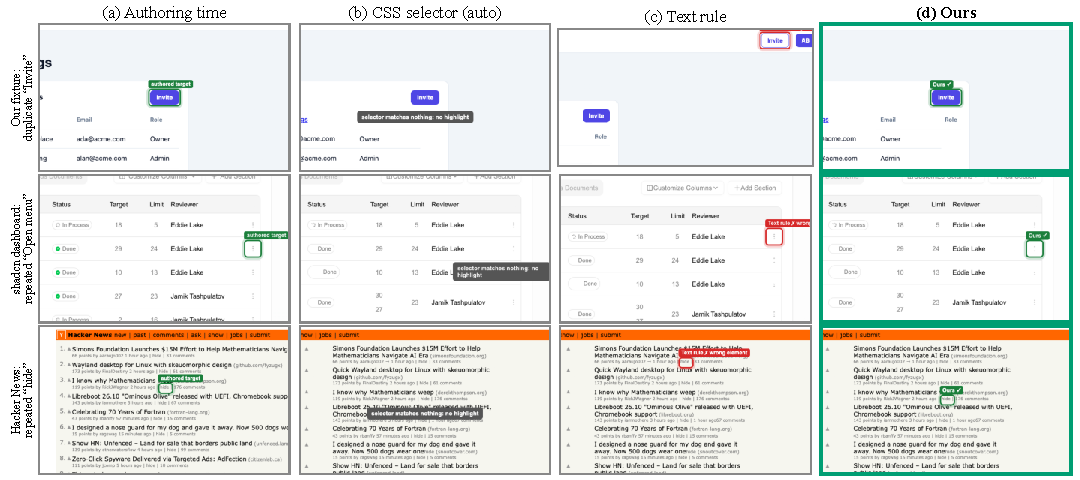
\includegraphics[width=\textwidth]{fig_hero.pdf}
\caption{\textbf{Same step, same redeployed page, four anchoring strategies.}
Each row authors a step on the pristine page (a), then re-resolves it after a composite
redeploy (class/ID renaming, wrapper drift, reordering, copy edits, injected duplicates; $\rho{=}0.5$).
(b)~A CSS selector generated by an off-the-shelf tool \cite{medv_finder} matches nothing, so the step silently fails.
(c)~A text rule finds the first control with the same label, which is a \emph{different} control (red).
(d)~Our v1 resolver re-scores every live element against a semantic descriptor and picks the intended one (green).
Examples are \emph{selected} to show the three behaviours side by side; aggregate results over
\nTrials{} resolutions are in Figs.~\ref{fig:robust}--\ref{fig:breakdown} and Table~\ref{tab:main}.}
\label{fig:hero}
\end{figure*}

\begin{abstract}
In-app guidance products, known as digital adoption platforms (DAPs), anchor each walkthrough step to a page element using a selector captured at authoring time. After a redeploy such an anchor either fails silently or, worse, points confidently at the wrong control.
We study this problem with a controlled benchmark of \nPages{} real and fixture page states under \nOps{} seeded perturbation operators, comparing our onboarding copilot against six locator strategies documented by commercial DAPs and the web-testing literature, including a Similo-style weighted-similarity matcher.
Our first resolver (v1, hand-weighted semantic scoring) is correct in \oursC\% of composite-redeploy resolutions, ahead of a role+name locator (\rnC\%) but well behind the Similo-style matcher (\simC\%); we report this plainly.
A learned listwise ranker over 20 locator and semantic features, with context features that compare each candidate with its competitors (v2), reaches \vTwoC\% correct and \vTwoW\% wrong on held-out pages (95\% CI \vTwoCci), statistically tied with the Similo-style matcher ($+\dCvSim$ points, CI \dCvSimLo{} to \dCvSimHi), and stays near 98\% correct under label edits on a perturbation type withheld from training.
A gradient-boosted ranker on the same features (v3) reaches \gbC\% correct and \gbW\% wrong on held-out pages (CI \gbCci), significantly ahead of the Similo-style matcher ($+\dCgb$ points correct, CI \dCgbLo{} to \dCgbHi; $-\dWgb$ points wrong). Margin-gated abstention cuts the wrong-highlight rate of our weaker v1 resolver by 40\%, with smaller gains for strong matchers.
On the real before/after data released with Similo (40 sites, 598 targets) a boosted ranker ties the original Similo code, and after a failure analysis, wording-robust features plus joint assignment give a modest but statistically significant gain (94.0\% against 90.1\% on 37 sites with identical targets), while a margin gate cuts its wrong-highlight rate to 2.6\% against 9.9\%. We also report the language-model compile-once architecture, measured runtime costs, and a defect the evaluation exposed in our own code.\end{abstract}

\begin{IEEEkeywords}
digital adoption platform, onboarding, web element localization, selective prediction, abstention, large language models, human-computer interaction.
\end{IEEEkeywords}

%% =====================================================================
\section{Introduction}\label{sec:intro}
Software products lose users who never reach their first valuable action. Digital adoption platforms try to prevent this by drawing tooltips and spotlights over an existing application without changing its source. The core operation is simple to state and hard to do well: given a step such as ``click \emph{Invite} in the Members section'', find that element on the live page. The vendors we reviewed (WalkMe, Whatfix, Pendo, Appcues, Userpilot, Userflow) describe the same basic answer in their help pages: capture an element or a selector while the flow is built and look it up again at run time \cite{walkme_what,pendo_css,appcues_selectors,userpilot_select,userflow_tooltip}.

Locators are known to be fragile. Hammoudi et al.\ catalogued 1{,}065 breakages of record/replay web tests across 453 versions of web applications and found locator problems among the main causes \cite{hammoudi2016}. Guidance has an additional hazard that tests do not. A broken test fails loudly, but a mis-anchored spotlight points confidently at the wrong control, and the user trusts it.

We study a copilot built around three ideas. First, a step carries a \emph{semantic descriptor} (role, accessible name, section, ordinal, and so on) that is re-scored against every live element on every tick, so nothing is cached that a re-render can invalidate. Second, a language model is used \emph{once per goal, offline}, as a compiler that emits a validated plan; at run time everything is deterministic and local. Third, the system is allowed to \emph{abstain}: when the evidence for a single element is weak, it shows text instead of a spotlight.

\textbf{Contributions.}
\begin{itemize}
\item \textbf{A controlled robustness benchmark for guidance anchors.} Eight seeded perturbation operators on \nPages{} real and fixture page states, with ground truth carried through every perturbation and metrics that separate \emph{wrong} highlights from \emph{abstentions} (Sec.~\ref{sec:protocol}).
\item \textbf{An honest head-to-head.} Our hand-weighted v1 resolver beats documented DAP locator strategies but \emph{loses} to a Similo-style weighted-similarity matcher; we show where and why.
\item \textbf{Learned local rankers (v2, v3).} A listwise linear ranker (v2) ties the strongest baseline on held-out pages and generalises to an unseen perturbation type; a gradient-boosted ranker (v3) on the same candidate-context features is significantly better than every baseline we ran, including a Similo-style matcher.
\item \textbf{Calibrated abstention and limits.} A margin gate calibrated on held-out pages, its measured benefit for each matcher, and an account of limits including a polling defect found in our own SDK.
\end{itemize}

%% =====================================================================
\section{Related Work}\label{sec:related}
\textbf{Commercial DAPs.}
Table~\ref{tab:daps} summarises the targeting behaviour that vendors document. WalkMe describes capturing an element by ID, position, text, or jQuery rule \cite{walkme_what}; its help pages list re-selecting the element or relaxing matching rules as the fix when an element is not found \cite{walkme_cant_find,walkme_advanced}. Whatfix labels captured elements strong or weak and suggests adding selector or text rules \cite{whatfix_visual}. Pendo offers suggested, parent, or custom CSS rules \cite{pendo_css}, and its community reports guides whose target matches several elements \cite{pendo_community}. Appcues stores a CSS selector at build time and asks authors to use stable attributes or edit the selector \cite{appcues_selectors,appcues_check}. Userpilot documents errors for dynamic IDs and iframes \cite{userpilot_select,userpilot_errors}, and Userflow asks for a manual selector when an element is not found \cite{userflow_tooltip}. In every case the documented remedy is an \emph{author edit}. Whatfix has also announced LLM-assisted authoring and agents that adapt to interface changes \cite{whatfix_ai,itbrief_whatfix}, which makes it the closest documented competitor. Documentation shows what a vendor states, not what it ships; we therefore do not benchmark vendor products, only the strategies they document (Sec.~\ref{sec:protocol}).

\begin{table*}[!t]
\caption{Targeting behaviour documented by six DAPs, and ours. ``Remedy'' is the fix the documentation prescribes.}
\label{tab:daps}
\centering\small
\begin{tabular}{@{}p{1.5cm}p{5.0cm}p{5.2cm}p{4.3cm}@{}}
\toprule
System & Targeting & Failure and documented remedy & AI features documented\\
\midrule
WalkMe \cite{walkme_what,walkme_cant_find} & Captured element: ID, position, text, jQuery & Element absent: re-select or relax matching & not reviewed\\
Whatfix \cite{whatfix_visual,whatfix_ai} & Captured element, strong/weak, CSS/jQuery & Weak element: add selector or text rule & LLM authoring, adaptive agents\\
Pendo \cite{pendo_css,pendo_community} & Suggested, parent, or custom CSS & Multiple matches: parent or custom CSS & not reviewed\\
Appcues \cite{appcues_selectors} & CSS selector saved at build time & Not unique/found: stable attributes or edit & not reviewed\\
Userpilot \cite{userpilot_select,userpilot_errors} & Auto CSS selector, optional text & Dynamic IDs, iframes: manual selector & not reviewed\\
Userflow \cite{userflow_tooltip} & Captured CSS class, ID, attribute & Not found: manual selector & not reviewed\\
\midrule
\textbf{Ours} & Semantic descriptor re-scored every tick; confidence gate & Below threshold: text-only guidance; telemetry; automatic recompile & One validated LLM call per goal, offline\\
\bottomrule
\end{tabular}
\end{table*}

\textbf{Robust element localization in web testing.}
The testing community has studied locator robustness for over a decade. ROBULA+ generates XPath locators that reduce fragility relative to absolute paths \cite{leotta2016robula}. Similo goes further and scores candidates by a weighted similarity over several locator attributes, locating the target in 89\% of 801 cases against 73\% for a baseline in the authors' study \cite{nass2023similo}. Similo is the closest relative of our scorer, so we include a Similo-style arm in our benchmark (our simplified reimplementation of weighted attribute similarity, not the authors' code), and we make no claim to have invented weighted multi-attribute matching. Later work extends Similo with visual-overlap groups (VON Similo) \cite{nass2023von}, an LLM re-ranking step \cite{nass2023llm}, and a hybrid of the two evaluated on a 23 times larger benchmark \cite{kluge2025relocalization}; a 2026 dataset collects reproducible locator breaks from open-source test suites \cite{reprobreak2026}. Their larger benchmarks and the LLM and hybrid variants are not released in a form we could run (the replication repository for \cite{kluge2025relocalization} omits the scraped site data), so we compare against the original Similo only. Our setting differs in three ways: the cost of a wrong answer is a confident misdirection rather than a failed test, so abstention is a first-class output; descriptors carry \emph{section context} derived from landmarks; and the resolver is part of a system that compiles, validates, caches, and repairs plans.

\textbf{LLM web agents.}
Mind2Web and SeeAct ask a language model to choose a page element for each action \cite{deng2023mind2web,zheng2024seeact}. SeeAct reports that grounding the model's plan to the right element is the main bottleneck. Putting the model on the hot path also adds a model call, with its latency and cost, to every step, and exposes every step to hallucination \cite{ji2023}. We take the opposite stance: the model runs once per goal, offline, picks among deterministically extracted candidates by id, and is validated.

\textbf{Reliability and abstention.}
The reject option \cite{chow1970} formalises the error--reject trade-off that our gates navigate. We adopt its evaluation view: report the correct, wrong, and abstained shares, and compare methods on the correct--wrong plane rather than on a single accuracy number.

\textbf{Position.}
To our knowledge, none of the DAPs whose documentation we reviewed documents the combination of semantic re-resolution on every tick, confidence-gated abstention, and a self-repairing compiled plan, and we are not aware of a published controlled evaluation of guidance-anchor robustness. Each element of the combination has precedent; the contribution is the combination and its measured behaviour.

%% =====================================================================
\section{Method}\label{sec:method}
\subsection{Overview}
\begin{figure*}[!t]
\centering
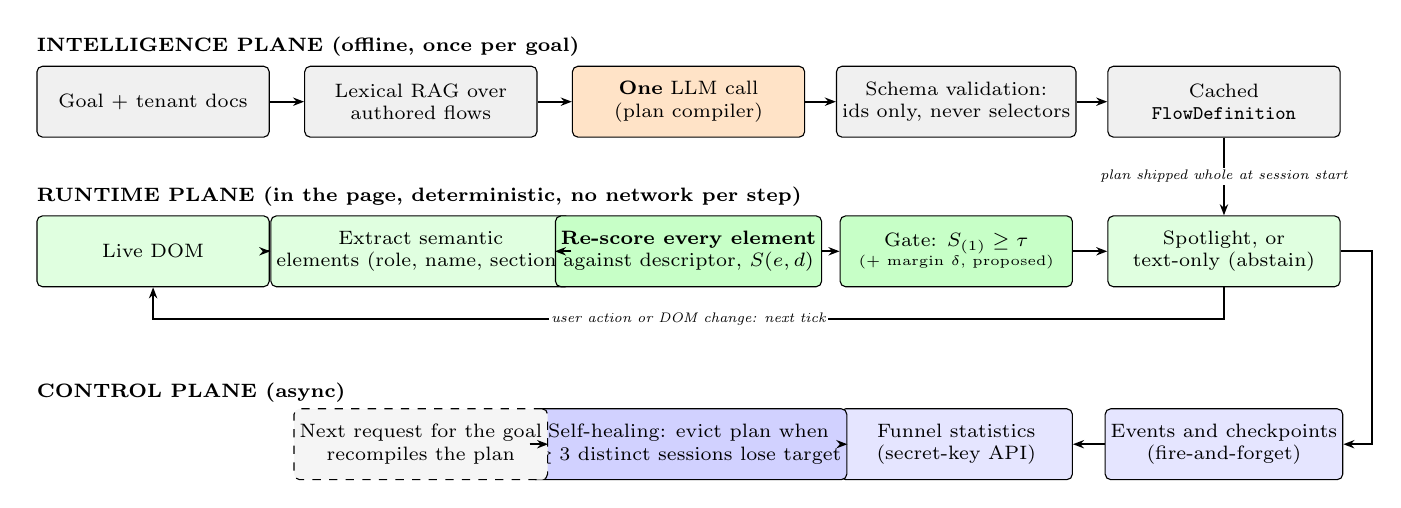
\begin{tikzpicture}[
  blk/.style={draw, rounded corners=2pt, align=center, font=\scriptsize, minimum height=9mm, minimum width=2.95cm, inner sep=2pt, fill=#1},
  blk/.default=white,
  arr/.style={-{Stealth[length=4pt]}, thick},
  plane/.style={font=\scriptsize\bfseries, anchor=west},
  lab/.style={font=\tiny\itshape, align=center, fill=white, inner sep=1pt}]
% Intelligence plane (offline)
\node[plane] at (0,3.55) {INTELLIGENCE PLANE (offline, once per goal)};
\node[blk=gray!12] (g) at (1.6,2.85) {Goal $+$ tenant docs};
\node[blk=gray!12] (r) at (5.0,2.85) {Lexical RAG over\\authored flows};
\node[blk=orange!22] (l) at (8.4,2.85) {\textbf{One} LLM call\\(plan compiler)};
\node[blk=gray!12] (z) at (11.8,2.85) {Schema validation:\\ids only, never selectors};
\node[blk=gray!12] (c) at (15.2,2.85) {Cached\\\texttt{FlowDefinition}};
\foreach \a/\b in {g/r,r/l,l/z,z/c}{\draw[arr] (\a) -- (\b);}
% Runtime plane
\node[plane] at (0,1.65) {RUNTIME PLANE (in the page, deterministic, no network per step)};
\node[blk=green!12] (d) at (1.6,0.95) {Live DOM};
\node[blk=green!12] (e) at (5.0,0.95) {Extract semantic\\elements (role, name, section)};
\node[blk=green!22] (s) at (8.4,0.95) {\textbf{Re-score every element}\\against descriptor, $S(e,d)$};
\node[blk=green!22] (t) at (11.8,0.95) {Gate: $S_{(1)}\ge\tau$\\[-1pt]{\tiny (+ margin $\delta$, proposed)}};
\node[blk=green!12] (u) at (15.2,0.95) {Spotlight, or\\text-only (abstain)};
\foreach \a/\b in {d/e,e/s,s/t,t/u}{\draw[arr] (\a) -- (\b);}
\draw[arr] (u.south) -- ++(0,-0.4) -| node[lab,pos=0.25] {user action or DOM change: next tick} (d.south);
% Control plane
\node[plane] at (0,-0.85) {CONTROL PLANE (async)};
\node[blk=blue!10] (ev) at (15.2,-1.5) {Events and checkpoints\\(fire-and-forget)};
\node[blk=blue!10] (fn) at (11.8,-1.5) {Funnel statistics\\(secret-key API)};
\node[blk=blue!18] (ev2) at (8.4,-1.5) {Self-healing: evict plan when\\$\ge 3$ distinct sessions lose target};
\node[blk=gray!8, dashed] (rc) at (5.0,-1.5) {Next request for the goal\\recompiles the plan};
\foreach \a/\b in {ev/fn,fn/ev2,ev2/rc}{\draw[arr] (\a) -- (\b);}
\draw[arr] (c) -- node[lab] {plan shipped whole at session start} (u);
\draw[arr] (u.east) -- ++(0.4,0) |- (ev.east);
\end{tikzpicture}
\caption{System overview. The language model appears exactly once, offline. Everything on the per-step path is a local, deterministic computation; telemetry flows back asynchronously and triggers recompilation when a cached plan keeps losing its target.}
\label{fig:arch}
\end{figure*}

Fig.~\ref{fig:arch} shows three planes. The \emph{runtime plane} runs inside the host page: it extracts a semantic view of the page, re-resolves the current step's target, and draws a spotlight or text-only card. The \emph{intelligence plane} turns a free-form goal and the tenant's documents into a validated plan with a single structured model call, cached per goal. The \emph{control plane} records events and evicts plans that keep failing. The compiled plan ships whole at session start, so the model is never called while a user is mid-guide.

\subsection{Semantic extraction}
Browsers expose no accessibility-tree API to in-page scripts, so the SDK computes one. For each interactive element it derives an ARIA role (explicit or implicit from the tag), an accessible name using a subset of the W3C algorithm \cite{w3c_accname}, a \emph{section label} (the accessible name of the nearest enclosing landmark), an \emph{ordinal} (index among elements sharing role and name), visibility, bounds, and a stable id (a hash of role, name, test id, section, structural path, and ordinal). Extraction keeps at most 250 elements per snapshot, visible-first; on pages with more than 500 interactive elements it first pre-selects the viewport-nearest candidates with one batched layout read.

\subsection{Descriptor scoring}
A step carries a descriptor $d$ holding the signals recorded when the element was authored. Let $I(d)$ be the signals that $d$ specifies, $f_i(e,d)\in[0,1]$ the match strength of signal $i$ on candidate $e$, and $w_i$ its weight. The score is normalised by the weight of the specified signals only, so a sparse descriptor is not penalised for omitting signals:
\begin{equation}
S(e,d)=v(e)\,\frac{\sum_{i\in I(d)} w_i\, f_i(e,d)}{\sum_{i\in I(d)} w_i},
\label{eq:score}
\end{equation}
where $v(e)$ is $0.5$ for a hidden element and $0.7$ for a disabled one (factors multiply). The weights in the shipped code are test id 1.0, name 0.9, \texttt{aria-label} 0.8, internal id 0.7, text 0.6, role 0.5, section 0.5, ordinal 0.3, ancestry 0.3, and bounding-box proximity 0.15. The best candidate is $e^{*}=\arg\max_e S(e,d)$.

The shipped code has two entry points. The \emph{plan executor} matches \emph{authored criteria} (role, exact name, optional section hint and test id) and draws a spotlight only if $S_{(1)}\ge\tau=0.6$ \emph{and} the section hint matches (a hard constraint):
\begin{equation}
\text{highlight} \iff S_{(1)}\ge\tau \;\wedge\; \text{section}(e^{*})\ \text{matches}.
\label{eq:gate}
\end{equation}
The \emph{runtime matcher} re-resolves the full descriptor of a displayed target every frame with a lower floor of $0.4$. We benchmark both paths. The existing ambiguity flag (top-two gap below $0.08$) only requests an optional AI tie-break; it does not suppress the highlight.

\subsection{Calibrated abstention (proposed)}
A confidence floor alone cannot tell a clear winner from a near-tie between two plausible elements. We therefore evaluate a \emph{margin gate}, which is \emph{not} in the shipped code:
\begin{equation}
\text{highlight} \iff S_{(1)}\ge\tau \;\wedge\; S_{(1)}-S_{(2)}\ge\delta.
\label{eq:margin}
\end{equation}
We select $\delta$ by two-fold cross-fitting over pages: for each fold, $\delta$ is the smallest value in $\{0.02,0.05,0.08,0.1,\dots\}$ that keeps the wrong-highlight rate at or below 5\% on the \emph{other} fold's composite-redeploy trials, and the gate is applied to the held-out fold. Both folds selected $\delta{=}\deltaGate$. This is the reject option of \cite{chow1970} applied to element resolution.

\subsection{Learned ranker (v2)}\label{sec:v2}
The v1 weights were set by hand. Borrowing from learning-to-rank, v2 treats resolution as a listwise choice among candidates. For each target we take all elements with the authored tag, keep the 15 best by a cheap prefilter, and describe every candidate with 20 features in $[0,1]$: Similo-style locator attributes (class, id, label, href, text, path, position, size, parent class, neighbour text) and our semantic signals (role, exact and fuzzy name, section, ordinal, visibility, test id). \emph{Context features} append, for each feature, the candidate's value minus the maximum and minus the mean over the candidate list, a one-layer analogue of the cross-candidate comparison that attention provides. Scores are linear, $s_j=\mathbf w^{\top}\phi_j$, and trained with a softmax cross-entropy over the list by L-BFGS. Inference is 60 multiply-adds per candidate, so once candidates are extracted the ranking costs microseconds; extraction, not ranking, dominates latency (Sec.~\ref{sec:results}). We deliberately did \emph{not} use a transformer: with 20 features and 15 candidates a linear listwise model is enough, exportable as one weight vector, and free of inference-time dependencies. Semantic text embeddings are the natural next step for wording changes.

\textbf{A boosted variant (v3).} A non-linear model can capture interactions that a linear score cannot, for example that a text match is decisive only when the position also agrees. v3 fits a gradient-boosted tree classifier (250 trees, 31 leaves, \texttt{HistGradientBoosting}) on the same context-augmented features, scoring each candidate pointwise and taking the argmax. In-browser latency of tree inference was not measured here; the model is small, but v3 is not yet integrated into the SDK.

\textbf{Evaluation protocol for v2 and v3.} To avoid fitting the benchmark, we use four-fold cross-validation over \emph{pages}: train on two folds, calibrate the margin gate $\delta$ on a third, and test on the fourth. Separately, a leave-one-operator-out run withholds each perturbation type from training and tests on it.

\subsection{Compile-once planning and self-healing}
Given a goal, the server tries authored flows (lexical retrieval), then a cached compiled flow, then makes \emph{one} structured model call (Gemini 2.5 Flash through the Vercel AI SDK, cf.~\cite{comanici2025}) grounded in knowledge chunks. The model sees a deterministic shortlist of at most eight candidates and returns an \emph{id}; every output is validated against a Zod schema, and an unknown id is rejected. A made-up identifier therefore cannot be rendered, but a wrong \emph{valid} candidate can; the scoring gates act as an independent deterministic check. A cached plan is evicted when $k{=}3$ distinct sessions report a lost target. If $n$ sessions fail independently with probability $p$, then $P_{\text{evict}}=\Pr[X\ge k]$ for $X\sim\mathrm{Bin}(n,p)$; for a broken plan ($p{=}0.5$, $n{=}10$) this is $0.945$, and for a healthy one ($p{=}0.01$, $n{=}100$) it is $0.079$ (analytic; the eviction logic is covered by unit tests, but we did not measure eviction on live traffic).

\subsection{Snapshot codec}
Runs of at least three structurally identical siblings are sent as one template plus per-instance deltas. If a group of $m$ elements has template size $s$ and per-instance delta $d_\Delta$, the compression ratio is $1/m+d_\Delta/s$. We measure real ratios in Sec.~\ref{sec:results}.

%% =====================================================================
\section{Experimental Protocol}\label{sec:protocol}
\subsection{Corpus and ground truth}
We use \nPages{} page states (Table~\ref{tab:corpus}): three states of our own hostile fixture (duplicate buttons, portal modal) and 27 public pages spanning admin dashboards, documentation, forms, and content sites (a 28th snapshot, the Internet Archive home page, yielded no eligible targets and is excluded). Each page is captured once as a self-contained MHTML snapshot with scripts removed, so every run starts from identical bytes, and is loaded in desktop Chrome. Before any perturbation, every element receives a hidden \texttt{data-gt} index. Perturbations carry the attribute with the node; clones injected as duplicates do not. \emph{No method reads it}: it is used only to score outcomes. A resolution is \emph{correct} if it returns the element with the authored index, \emph{wrong} if it returns another element, and an \emph{abstention} if it returns nothing.

\begin{table}[!t]
\caption{Corpus. ``Targets'' is the number of eligible target elements (visible, enabled, named; \emph{of which} up to 10 are sampled); ``Dup.'' counts those sharing role and accessible name with another element.}
\label{tab:corpus}
\centering\scriptsize
\begin{tabular}{@{}p{4.6cm}lrr@{}}
\toprule
Page state & Type & Targets & Dup.\\
\midrule
Our fixture: dashboard & Fixture & 14 & 0 \\
Our fixture: members settings & Fixture & 14 & 2 \\
Our fixture: invite modal open & Fixture & 17 & 2 \\
AdminLTE 3 dashboard demo \cite{page_adminlte} & Admin UI & 33 & 6 \\
AdminLTE general forms \cite{page_adminlte_forms} & Forms & 73 & 23 \\
AdminLTE data tables \cite{page_adminlte_tables} & Admin UI & 44 & 10 \\
Angular home \cite{page_angular_dev} & Docs & 48 & 2 \\
Bootstrap checkout example \cite{page_bootstrap_checkout} & Forms & 25 & 0 \\
Bootstrap dashboard example \cite{page_bsdash} & Admin UI & 18 & 0 \\
Bootstrap forms overview \cite{page_bsforms} & Forms & 167 & 39 \\
Bootstrap navbar component docs \cite{page_bootstrap_navbar} & Docs & 247 & 110 \\
Bootstrap pricing example \cite{page_bootstrap_pricing} & Web app & 23 & 0 \\
Bootstrap sign-in example \cite{page_bootstrap_signin} & Forms & 5 & 0 \\
Django documentation \cite{page_django_docs} & Docs & 226 & 38 \\
Flask documentation \cite{page_flask_docs} & Docs & 249 & 45 \\
GitHub repository page \cite{page_github} & Web app & 201 & 54 \\
Hacker News front page \cite{page_hn} & Content & 187 & 57 \\
MDN \texttt{<button>} reference \cite{page_mdn} & Docs & 250 & 38 \\
Next.js documentation \cite{page_nextjs_docs} & Docs & 108 & 39 \\
PyPI home \cite{page_pypi} & Web app & 54 & 7 \\
Python 3 documentation \cite{page_pydocs} & Docs & 78 & 47 \\
React documentation home \cite{page_react} & Docs & 122 & 60 \\
shadcn/ui dashboard example \cite{page_shadcn} & Admin UI & 118 & 55 \\
shadcn/ui tasks example \cite{page_shadcn_tasks} & Admin UI & 89 & 55 \\
Svelte home \cite{page_svelte_dev} & Docs & 126 & 9 \\
Tailwind CSS installation docs \cite{page_tailwind_docs} & Docs & 234 & 35 \\
TodoMVC (React) \cite{page_todomvc} & Web app & 12 & 2 \\
Vue.js home \cite{page_vuejs} & Docs & 56 & 42 \\
W3C home \cite{page_w3c} & Content & 47 & 7 \\
Wikipedia main page \cite{page_wiki} & Content & 229 & 24 \\
\bottomrule
\end{tabular}
\end{table}

\subsection{Authoring and perturbations}
For each page we author \nTargets{} targets once, on the pristine DOM, taking the descriptor that the SDK derives from the element (as a recorder would) and, for the criteria path, a role, exact name, and the element's own section and test id when present. Up to three targets per page are chosen among elements that have a same-named twin, so the hard cases are always represented. Table~\ref{tab:ops} lists the operators; each takes an intensity $\rho\in\{0.1,0.25,0.5,0.75,1\}$ that sets the fraction of eligible nodes affected, and each is run with \nSeeds{} seeds. Class and ID renames also rewrite the page's stylesheets so the layout is preserved. The composite \emph{redeploy} mimics a release that changes several things at once.

\begin{table}[!t]
\caption{Perturbation operators.}
\label{tab:ops}
\centering\scriptsize
\begin{tabular}{@{}p{1.9cm}p{3.5cm}p{1.9cm}@{}}
\toprule
Operator & Action & Probes\\
\midrule
Class rename & Rename CSS classes (and stylesheet rules) & class selectors\\
ID randomisation & Replace ids; fix \texttt{for}, \texttt{aria-*}, \texttt{href\#} & id selectors\\
DOM reorder & Shuffle siblings of random parents & positions, ordinals\\
Wrapper drift & Insert layout-neutral wrappers and hidden siblings & paths, nth-child\\
Copy drift & Suffix, prefix, upper-case, or pluralise labels & text, name rules\\
Dup.\ (other sect.) & Clone the target into another container & non-unique matches\\
Dup.\ (adjacent) & Clone the target next to itself & inherent ambiguity\\
Composite redeploy & Classes $\rho$, ids $\rho$, wrappers $0.5\rho$, copy $0.35\rho$, reorder $0.3\rho$, dup.\ $0.3\rho$ & all of the above\\
\bottomrule
\end{tabular}
\end{table}

\subsection{Methods}
Table~\ref{tab:methods} lists the arms. The first seven are \emph{our implementations of the strategies that the DAP documentation and testing literature describe}; they are not the vendors' products, whose internals we cannot inspect. The CSS arm uses an independent open-source selector generator \cite{medv_finder} rather than code we wrote.

\begin{table}[!t]
\caption{Methods. Baselines emulate documented strategies; they are not vendor products.}
\label{tab:methods}
\centering\scriptsize
\begin{tabular}{@{}p{2.0cm}p{3.7cm}p{1.6cm}@{}}
\toprule
Arm & Resolution rule & Family\\
\midrule
CSS selector & generated by \texttt{finder} \cite{medv_finder}, DOM lookup & Appcues, Userpilot, Userflow, Pendo\\
XPath & absolute positional path & position capture\\
Text rule & first same-tag element with identical text & WalkMe, Whatfix text rules\\
Selector chain & id $\to$ CSS $\to$ text $\to$ XPath, first hit & multi-rule fallback\\
Role+name & first element with same role and accessible name & Playwright \cite{playwright_locators}\\
Role+name (strict) & as above, abstain if not unique & Playwright strict mode\\
Similo-style & argmax of weighted attribute similarity (tag, class, id, label, href, text, path, position, size); never abstains & Similo \cite{nass2023similo}\\
\midrule
Ours v1 (criteria) & Authored criteria, Eq.~\eqref{eq:gate} & shipped plan executor\\
Ours v1 & Full descriptor, Eq.~\eqref{eq:score}, $\tau{=}0.6$ & shipped matcher\\
Ours v2 & Learned listwise ranker, Sec.~\ref{sec:v2}, page-held-out & proposed\\
Ours v3 & Boosted-tree ranker, same features, page-held-out & proposed\\
$+$ margin & Eq.~\eqref{eq:margin}, held-out $\delta$ & proposed\\
\bottomrule
\end{tabular}
\end{table}

\subsection{Metrics and statistics}
We report the correct rate $C$, wrong-highlight rate $W$, and abstain rate $A$ ($C{+}W{+}A=1$), plus precision $C/(C{+}W)$. Trials within a page are correlated, so confidence intervals use a \emph{cluster bootstrap over pages} \cite{efron1979}, not a binomial interval over resolutions. Paired differences resample the same pages for both methods. Headline numbers pool the composite redeploy at $\rho\in\{0.5,1\}$ ($n{=}1{,}400$ resolutions per method). The benchmark records \nRows{} outcomes in total.

%% =====================================================================
\section{Results}\label{sec:results}
\subsection{Main comparison}
Table~\ref{tab:main} and Fig.~\ref{fig:breakdown} compare all arms under composite redeploys. The structural baselines (CSS, XPath) rarely survive a redeploy but \emph{fail loudly}: they abstain in \cssA\% and \xpA\% of cases and are wrong in about 5--6\%. The always-answer baselines that look at text or names (text rule, selector chain, role+name) are correct in at most \rnC\% and wrong in \rnW--\chainW\% of cases.

\textbf{Our v1 resolver beats those but not the strongest baseline.} It is correct in \oursC\% and wrong in \oursW\% (CI \oursWci), better than role+name by \dCrn{} points correct and \dWrn{} points fewer wrong (both CIs exclude zero). But the Similo-style weighted-similarity matcher, which blends many locator attributes, is correct in \simC\% and wrong in \simW\%, i.e., \dCsim{} points better than v1 on correct (CI \dCsimLo--\dCsimHi). v1 matches names exactly and leans on a positional ordinal hint, and it uses few of the attributes (class, href, path, position, neighbours) that survive a redeploy.

\textbf{Our learned v2 ranker closes the gap.} Trained on other pages only, v2 is correct in \vTwoC\% (CI \vTwoCci) and wrong in \vTwoW\% (CI \vTwoWci). Against the Similo-style matcher the paired difference is $+\dCvSim$ points correct (CI \dCvSimLo{} to \dCvSimHi) and $\dWvSim$ points wrong: a statistical tie, not a win (v3, below, does better). Against v1 it is a large gain, and against role+name it is $+27.5$ points correct. \textbf{A boosted ranker (v3) goes further.} With the same features, v3 is correct in \gbC\% (CI \gbCci) and wrong in \gbW\% (CI \gbWci). Against the Similo-style matcher the paired differences are $+\dCgb$ points correct (CI \dCgbLo--\dCgbHi) and $-\dWgb$ points wrong (CI \dWgbLo--\dWgbHi), both excluding zero, so on this benchmark v3 is significantly better than every baseline we ran. The margin gate changes little for v2 (\vTwomC\% correct, \vTwomW\% wrong), because a strong ranker leaves few near-ties to abstain on.

\begin{table*}[!t]
\caption{Composite redeploy, pooled over $\rho\in\{0.5,1\}$ (percent; 95\% cluster-bootstrap CIs over pages in brackets). $C$: correct highlight; $W$: wrong highlight; $A$: abstain; Prec.: $C/(C{+}W)$. Bold marks the best $C$ and the lowest $W$; the lowest $W$ is achieved by abstaining often. $^{\dagger}$Proposed, not shipped; $\delta$ chosen on held-out pages.}
\label{tab:main}
\centering\small
\begin{tabular}{@{}lrlrlrr@{}}
\toprule
Method & $C\uparrow$ & & $W\downarrow$ & & $A$ & Prec.\\
\midrule
CSS selector (auto) & 11.3 & {\scriptsize[8.7, 14.0]} & 6.2 & {\scriptsize[3.7, 9.0]} & 82.5 & 64.4\\
XPath (absolute) & 8.5 & {\scriptsize[6.0, 11.2]} & 4.6 & {\scriptsize[2.9, 6.5]} & 86.8 & 64.9\\
Text rule & 57.1 & {\scriptsize[50.9, 62.8]} & 32.4 & {\scriptsize[26.0, 40.0]} & 10.4 & 63.8\\
Selector chain & 58.2 & {\scriptsize[53.0, 63.2]} & 34.2 & {\scriptsize[28.6, 40.1]} & 7.6 & 63.0\\
Role+name (first) & 66.1 & {\scriptsize[60.9, 71.2]} & 21.4 & {\scriptsize[17.0, 26.4]} & 12.6 & 75.6\\
Role+name (strict) & 49.8 & {\scriptsize[44.4, 55.2]} & \textbf{3.0} & {\scriptsize[2.1, 4.2]} & 47.2 & 94.3\\
Similo-style (our reimpl.) & 93.6 & {\scriptsize[90.8, 96.0]} & 6.4 & {\scriptsize[4.0, 9.2]} & 0.0 & 93.6\\
Similo-style + margin gate$^{\dagger}$ & 92.0 & {\scriptsize[89.2, 94.8]} & 5.0 & {\scriptsize[2.7, 7.7]} & 3.0 & 94.9\\
\midrule
Ours v1, authored criteria & 29.3 & {\scriptsize[21.6, 38.4]} & 5.0 & {\scriptsize[2.5, 7.9]} & 65.7 & 85.5\\
Ours v1 (hand-weighted) & 72.2 & {\scriptsize[67.0, 76.6]} & 9.7 & {\scriptsize[7.5, 12.3]} & 18.1 & 88.2\\
Ours v1 + margin gate$^{\dagger}$ & 70.7 & {\scriptsize[65.9, 75.1]} & 5.9 & {\scriptsize[3.8, 8.1]} & 23.4 & 92.3\\
\midrule
Ours v2 (learned ranker) & 94.4 & {\scriptsize[92.3, 96.5]} & 5.6 & {\scriptsize[3.5, 7.7]} & 0.0 & 94.4\\
Ours v2 + margin gate$^{\dagger}$ & 93.8 & {\scriptsize[91.5, 96.0]} & 5.2 & {\scriptsize[3.3, 7.2]} & 1.0 & 94.8\\
\midrule
Ours v3 (boosted ranker) & \textbf{96.3} & {\scriptsize[93.9, 98.2]} & 3.7 & {\scriptsize[1.8, 6.1]} & 0.0 & 96.3\\
Ours v3 + margin gate$^{\dagger}$ & 96.1 & {\scriptsize[93.7, 98.0]} & 3.7 & {\scriptsize[1.7, 6.0]} & 0.2 & 96.3\\
\bottomrule
\end{tabular}
\end{table*}

\begin{figure*}[!t]
\centering
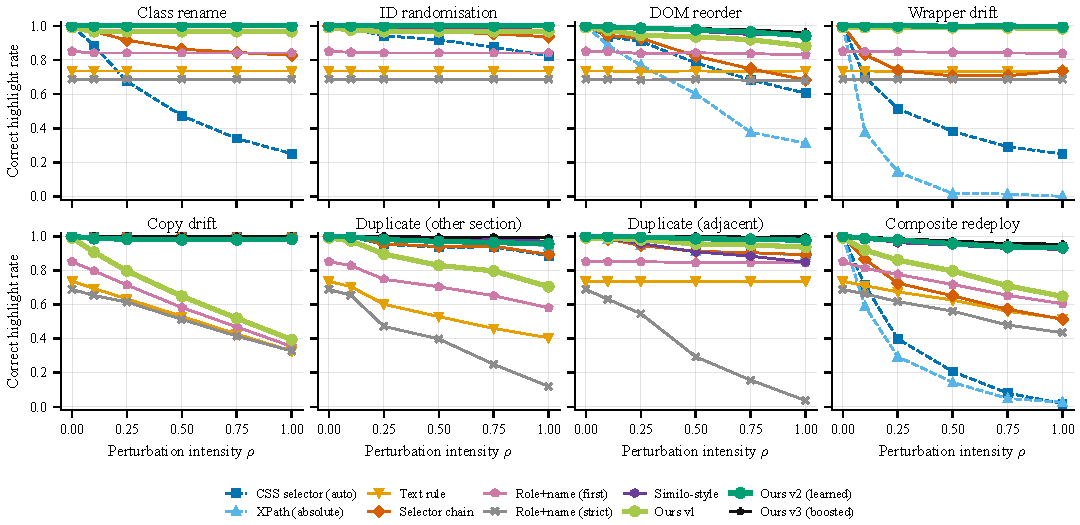
\includegraphics[width=\textwidth]{fig_robust_correct.pdf}
\caption{Correct-highlight rate against perturbation intensity $\rho$ for each operator (identity at $\rho{=}0$). Structural baselines (dashed blue) are unaffected by copy drift but collapse under class, wrapper, and composite changes. Our v1 resolver (light green) degrades gracefully but loses ground under copy drift; the learned v2 ranker (dark green) and the Similo-style matcher stay near the top throughout.}
\label{fig:robust}
\end{figure*}

\begin{figure*}[!t]
\centering
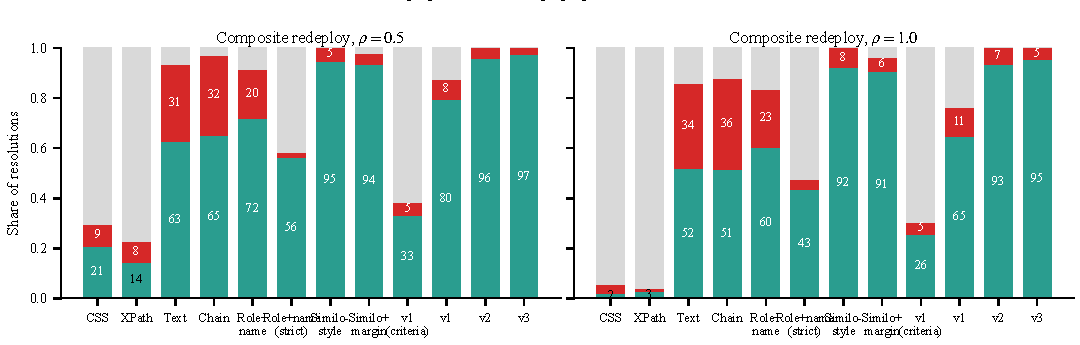
\includegraphics[width=\textwidth]{fig_breakdown.pdf}
\caption{Where each method's resolutions go under composite redeploy: correct, \emph{wrong} (red), or abstain. Percentages are shown for the correct and wrong segments.}
\label{fig:breakdown}
\end{figure*}

\subsection{Where we win, and where we do not}
Table~\ref{tab:opsres} lists $C/W$ per operator at $\rho{=}1$ (v2 and v3 are page-held-out). Three patterns stand out. First, label edits (copy drift) cut v1 and the role+name locator to roughly a third correct, while v2 and the Similo-style matcher stay near 98\% because they rely on many non-text signals and v2 has fuzzy name features; structural selectors are unaffected. Second, injected duplicates are the hardest case for every method: with a same-named twin present, role+name is wrong in 57\% of composite-redeploy resolutions, v1 in 20\%, Similo-style in 16\%, and v2 in 12\%. Third, DOM reordering is where the structural baselines collapse and the matchers that carry context hold up. In a \emph{leave-one-operator-out} run (each operator withheld from training), v2 stays at 94\% correct under reordering, 98\% under copy drift and 93\% under the composite redeploy, so the learned weights are not tied to the operators they were fit on.

\begin{table*}[!t]
\caption{Correct/wrong percent at $\rho{=}1$ for each operator. Bold marks the highest correct rate in each row.}
\label{tab:opsres}
\centering\scriptsize
\setlength{\tabcolsep}{3.2pt}
\begin{tabular}{@{}lccccccccc@{}}
\toprule
Operator & CSS & XPath & Text & Chain & Role+name & Similo & Ours v1 & Ours v2 & Ours v3\\
\midrule
Identity ($\rho{=}0$) & \textbf{100/0} & \textbf{100/0} & 74/26 & \textbf{100/0} & 85/14 & \textbf{100/0} & 99/0 & \textbf{100/0} & \textbf{100/0}\\
\midrule
Class rename & 25/0 & \textbf{100/0} & 74/26 & 83/17 & 84/15 & \textbf{100/0} & 97/0 & \textbf{100/0} & \textbf{100/0}\\
ID randomisation & 82/0 & \textbf{100/0} & 74/26 & 94/6 & 84/15 & 100/0 & 97/0 & \textbf{100/0} & \textbf{100/0}\\
DOM reorder & 61/29 & 31/25 & 74/26 & 68/32 & 83/14 & 95/5 & 88/7 & 94/6 & \textbf{96/4}\\
Wrapper drift & 25/11 & 0/0 & 73/27 & 74/26 & 84/15 & 99/1 & 98/0 & 99/1 & \textbf{100/0}\\
Copy drift & \textbf{100/0} & \textbf{100/0} & 33/20 & \textbf{100/0} & 35/13 & 98/2 & 39/4 & 98/2 & 100/0\\
Dup. (other section) & 89/10 & 94/6 & 40/59 & 89/11 & 58/40 & 97/3 & 70/27 & 95/5 & \textbf{99/1}\\
Dup. (adjacent) & 89/11 & 89/11 & 74/26 & 89/11 & 84/14 & 85/15 & 94/4 & 98/2 & \textbf{100/0}\\
Composite redeploy & 2/3 & 3/1 & 52/34 & 51/36 & 60/23 & 92/8 & 65/11 & 93/7 & \textbf{95/5}\\
\bottomrule
\end{tabular}
\end{table*}

\begin{figure*}[!t]
\centering
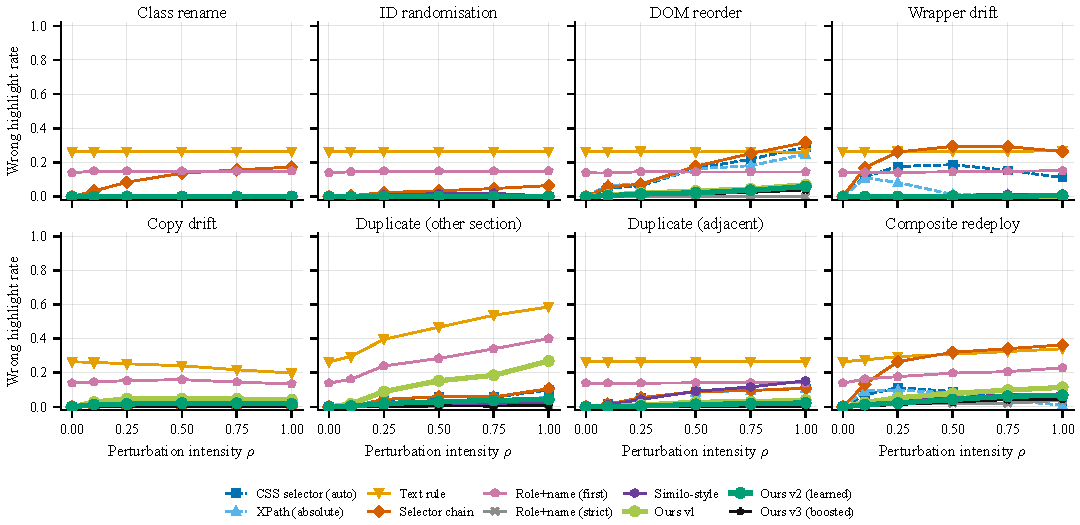
\includegraphics[width=\textwidth]{fig_robust_wrong.pdf}
\caption{Wrong-highlight rate against intensity. Always-answer baselines (text rule, chain, role+name) accumulate wrong highlights as the page drifts; abstaining methods stay near zero by giving up coverage.}
\label{fig:robustwrong}
\end{figure*}

\subsection{Risk--coverage and the margin gate}
The shipped confidence floor barely moves v1's operating point: between $\tau{=}0.4$ and $0.6$ its correct rate changes by about one point. A margin gate does more. For v1 it lowers the wrong-highlight rate from \oursW\% to \marginW\% (CI \marginWci) at a modest cost in coverage. For the strong matchers the gain is small, because there is little error left to remove (Similo-style: \simW\% to \simmW\%; v2: \vTwoW\% to \vTwomW\%). Fig.~\ref{fig:riskcov} places every method on the correct--wrong plane: abstention is most valuable for weak matchers and is a cheap safety net for strong ones.

\begin{figure}[!t]
\centering
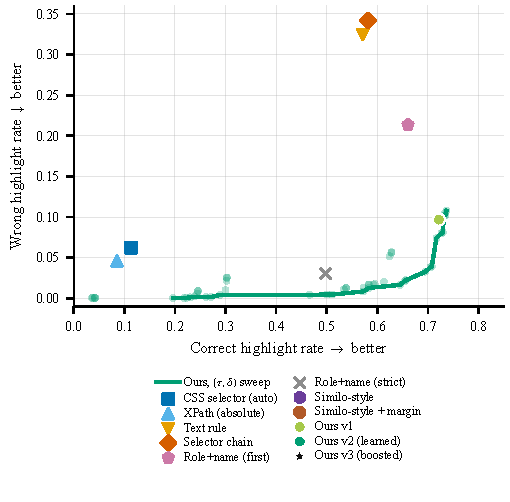
\includegraphics[width=0.92\columnwidth]{fig_riskcov.pdf}
\caption{Correct against wrong-highlight rate (composite redeploy, $\rho\in\{0.5,1\}$). Lower right is better. The green curve sweeps $(\tau,\delta)$ for our resolver; markers are baselines. The star is the held-out margin gate.}
\label{fig:riskcov}
\end{figure}

\subsection{Ablation}\label{sec:abl}
Table~\ref{tab:abl} removes signals from the v1 descriptor. Context matters: role and name alone raise the wrong-highlight rate to about 19\%. But removing the \emph{section and ordinal hints together} slightly \emph{improves} v1's pooled result, because the ordinal is positional and brittle under reordering and duplicate injection. This was an early signal that v1's hand-set weights were wrong, and it motivated learning them (Sec.~\ref{sec:v2}); the learned v2 weights down-weight neither hint to zero but rely mostly on position, href, text, and neighbouring text.

\begin{table}[!t]
\caption{Descriptor ablation, composite redeploy pooled (percent).}
\label{tab:abl}
\centering\scriptsize
\begin{tabular}{@{}lrrr@{}}
\toprule
Variant & $C$ & $W$ & $A$\\
\midrule
Full descriptor (shipped) & 72.2 & 9.7 & 18.1\\
$-$ section \& ordinal hints & 75.3 & 8.4 & 16.2\\
$-$ bounding-box hint & 70.3 & 9.7 & 20.1\\
$-$ internal id & 73.4 & 10.5 & 16.1\\
$-$ all context (role, name, text, test id) & 65.6 & 18.6 & 15.8\\
role + name only & 65.1 & 19.2 & 15.7\\
\bottomrule
\end{tabular}
\end{table}

\begin{figure}[!t]
\centering
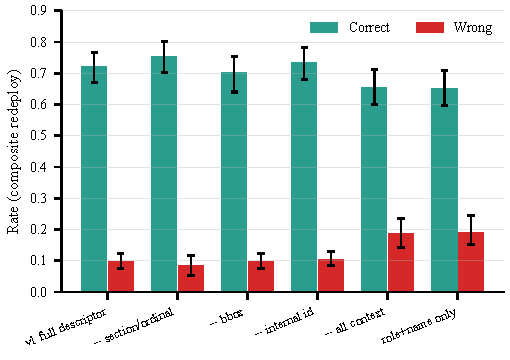
\includegraphics[width=0.92\columnwidth]{fig_ablation.pdf}
\caption{Ablation with 95\% cluster-bootstrap intervals. Removing all context nearly doubles wrong highlights.}
\label{fig:abl}
\end{figure}

\subsection{Real before/after benchmark: the Similo replication package}\label{sec:real}
Synthetic perturbations are a limitation, so we also ran on the \emph{real} dataset released with Similo \cite{nass2023similo}: 48 websites with the target element in an old version and all candidates in the new version, with the authors' own per-site outputs for XPath, Selenium IDE, ROBULA+, Montoto, Multilocator, and Similo from their original code. Eight sites ship without their element files, leaving 40 sites and 598 targets; we recompute every published baseline on exactly this subset. Our rankers use the dataset's locator attributes as features, are trained on other sites only (five folds by site), and CIs are bootstrapped over sites.

Table~\ref{tab:real} gives the result. \textbf{We do not beat the original Similo here.} Our boosted ranker is correct in 88.9\% against 90.1\% for Similo ($-1.2$ points, 95\% CI -5.1 to 3.1), a tie, and well above ROBULA+, Montoto, Selenium IDE, and Multilocator. The margin gate trades coverage for safety: it cuts wrong highlights from 9.9\% to 5.4\% ($-4.6$ points, CI -9.0 to -1.2) at the cost of abstaining on 11.7\% of targets and $-7.2$ points of correct rate. Feeding each confirmed outcome back into the matcher (an online update after every guided step, evaluated predict-then-learn) improved the linear ranker by only 0.2 points (CI 0.0 to 0.6): streams of about 15 targets per site are too short for the feedback loop to matter, so we do not claim a benefit. A further idea that does help is \emph{joint assignment}: because each new element can match at most one old target on a site, solving all of a site's targets together with the Hungarian algorithm raises the linear ranker from 91.6\% to 92.7\% correct ($+1.2$ points, CI 0.4 to 2.0). Against Similo's 90.1\% this is $+2.7$ points with an interval (\,$-0.4$ to $+6.8$) that includes zero. \textbf{Failure-driven features.} A failure analysis of the remaining errors showed that most (78\%, 40 of 51) were targets whose text had changed or vanished, which string-overlap features cannot handle. Adding wording-robust features, namely normalised compression distance over all attributes and token-level overlap of class, href, text, neighbours, and labels, lifts the linear ranker, and with joint assignment it beats Similo on identical targets. To make the comparison exact we restrict to the 37 sites where our parsed target count equals Similo's tabulated count (548 targets; three sites differ because the authors filtered some targets). There the joint ranker is correct in \textbf{94.0\% against Similo's 90.1\%} ($+4.0$ points, 95\% CI $+0.4$ to $+8.3$ over sites; one-at-a-time 92.5\%). With the margin gate it is wrong on only 2.6\% of targets (abstaining on 8.6\%) against Similo's 9.9\% ($-7.5$ points, CI $-12.5$ to $-4.0$), at a correct rate (88.9\%) statistically indistinguishable from Similo's. Because the features were motivated by error analysis on these same sites, we checked replication on disjoint halves of the sites: the gain is $+3.8$ points on one half (19 sites) and $+4.4$ on the other (18 sites), each with a wider interval because of half the data, and in both halves 80--83\% of failures are changed-text targets, so the mechanism replicates. All fits use held-out sites. The remaining limit is that this is a single dataset. We also tried pretraining on 25{,}000 synthetic-benchmark groups using the nine features the two datasets share: this gave 86.6\% correct against 85.6\% without pretraining, both below Similo's 90.1\% (a negative result we keep, since the shared-feature subset discards the signals that make Similo strong).

\textbf{What did not help (a broad sweep).} To test whether the 94.0\% is a modelling ceiling, we tried a wide set of ideas on the 37 matched sites, all with held-out sites. A set-transformer that attends over the candidate set, a listwise MLP, and their ensemble reach 91.4\%, 92.0\%, and 92.2\%, no better than the linear model. Combining the ranker with temperature scaling, dual-softmax agreement between targets and candidates, Sinkhorn optimal transport, stable (Gale--Shapley) matching, per-site self-training, and a linear-plus-boosted ensemble all plateau at or below 94.0\%, the value joint assignment alone gives. Adversarial augmentation that masks the text signals during training does not help (93.1--94.0\%), and neither do fly-olfaction-inspired features, in which each element's attributes are hashed by sparse random expansion and winner-take-all \cite{dasgupta2017fly} (93.6\%); a seven-feature model built on them reaches 92.2\%, close to Similo but not above it. Two further modern techniques did not help either: VON-style evidence from visually overlapping elements \cite{nass2023von} (93.2\%) and pretrained sentence embeddings of text, labels, and neighbours (93.1\%). We read this as evidence that the remaining errors are limited by the information in the attributes (for example targets whose text and position both changed), not by the optimiser or the architecture.

\textbf{Per-site view and the matcher's skeleton.} Fig.~\ref{fig:siteheat} shows, for each of the 37 real websites, the correct rate of every published baseline (from the authors' tables), of Similo, and of our one-by-one and joint rankers. Our joint ranker is better than Similo on 15 sites, tied on 17, and worse on 5 (Intuit $-36$ points, Zillow $-22$, Amazon $-10$, Indeed $-8$, Twitter $-5$); the baselines that rely on a single locator (XPath, Id-XPath) score zero on most sites. Fig.~\ref{fig:featheat} is the learned matcher's ``skeleton'': the signals with the largest total weight are word-level text overlap, text similarity, compression distance of the text, the id-based path similarity, the tag, position, and XPath similarity, which matches the failure analysis (text drift dominates the errors). Fig.~\ref{fig:skeleton} paints every element of three real pages by the probability our matcher assigns to it: probability mass concentrates on the true target (green) even where Similo picks a neighbour (red dashed), though it can be low (Amazon, $P{=}0.16$), where the margin gate abstains.

\textbf{Fresh sites, zero-shot.} To test beyond the 40 sites we built a new before/after set from Internet Archive snapshots of sites not in Similo's data (Python, W3C, Apache, Debian, Ubuntu, Mozilla, GNU), labelling ground truth from anchors that are then removed from every method's input (link target, or id), and keeping only targets whose XPath changed. We first checked our exact port of Similo's scoring (weights and similarity functions from the authors' Java source) on the original dataset: it scores 89.1\% against the 90.1\% the authors report, so we use it as the Similo baseline on the new data. The Internet Archive throttled our crawler, so the new set is small: with 2021 versus 2025 snapshots (4 sites, 92 targets) both methods are saturated (Similo 98.9\%, ours 100\%), and with 2017 versus 2025 snapshots (3 sites, 67 targets) ours scores 92.5\% against 91.0\% ($+1.7$ points, CI $0.0$ to $+5.0$), trained only on the original sites. This confirms the direction on unseen sites but is too small to be evidence by itself.

\begin{figure*}[!t]
\centering
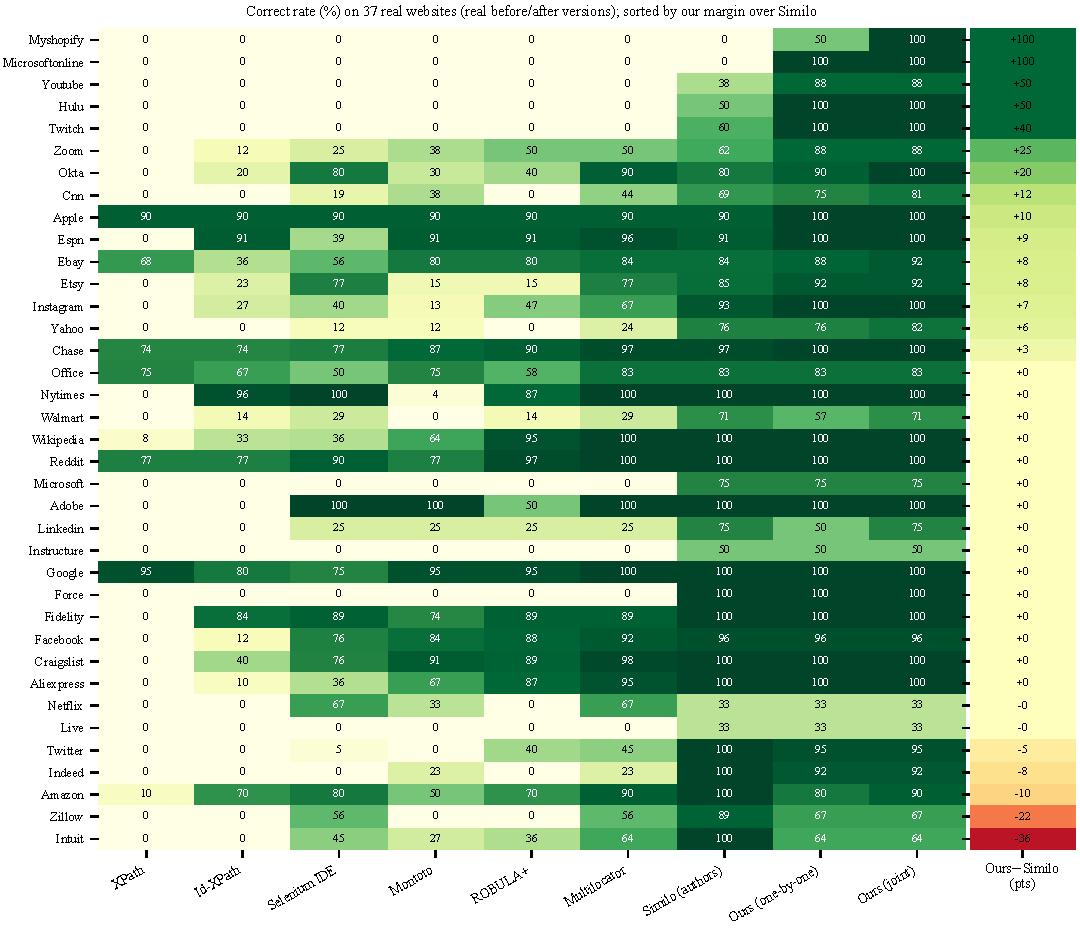
\includegraphics[height=0.62\textheight,keepaspectratio]{fig_site_heatmap.pdf}
\caption{Per-website correct rate on the 37 real before/after sites: published baselines, Similo, and ours (held-out sites). Rows are sorted by our margin over Similo (right column); green rows at the top are where we outperform, red rows at the bottom where we lose.}
\label{fig:siteheat}
\end{figure*}

\begin{figure*}[!t]
\centering
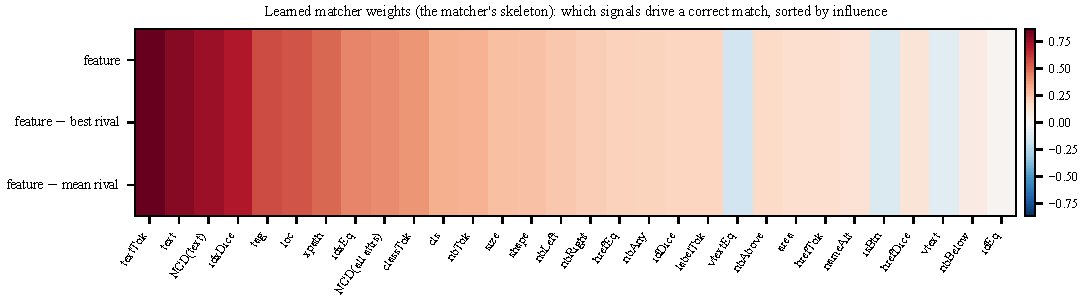
\includegraphics[width=\textwidth]{fig_feature_heatmap.pdf}
\caption{Learned matcher weights over the 30 locator and semantic features, with context variants (feature minus the best and mean rival candidate). Text-drift-robust signals dominate.}
\label{fig:featheat}
\end{figure*}

\begin{figure*}[!t]
\centering
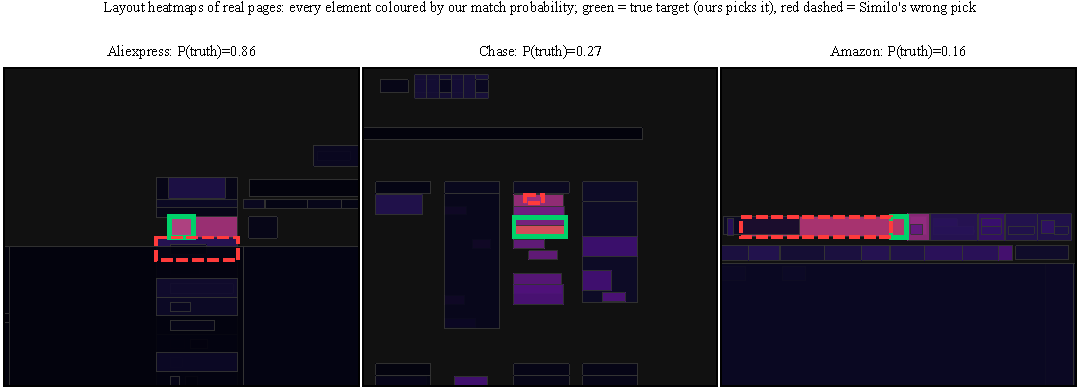
\includegraphics[width=\textwidth]{fig_skeleton.pdf}
\caption{Layout heatmaps of three real pages (zoomed on the target): every element is coloured by the probability our matcher assigns to it. The true target is outlined green; Similo's wrong pick is red dashed.}
\label{fig:skeleton}
\end{figure*}

\begin{table}[!t]
\caption{Real before/after data (Similo replication package, 40 sites, 598 targets; percent). Baseline rows are the authors' published outputs; $W$ is wrong, $A$ is not found/abstain. $^{\dagger}$Proposed.}
\label{tab:real}
\centering\scriptsize
\begin{tabular}{@{}lrlrr@{}}
\toprule
Method & $C$ & & $W$ & $A$\\
\midrule
XPath & 20.9 & {\scriptsize[9.1, 34.5]} & 3.0 & 76.1\\
Id-XPath & 40.8 & {\scriptsize[26.9, 53.6]} & 7.4 & 51.8\\
Selenium IDE & 53.3 & {\scriptsize[41.9, 63.4]} & 6.2 & 40.5\\
Montoto & 54.3 & {\scriptsize[40.0, 65.3]} & 1.3 & 44.3\\
ROBULA+ \cite{leotta2016robula} & 64.5 & {\scriptsize[50.0, 75.2]} & 4.0 & 31.4\\
Multilocator & 76.1 & {\scriptsize[64.0, 84.7]} & 0.0 & 23.9\\
Similo (authors' code) \cite{nass2023similo} & 90.1 & {\scriptsize[84.4, 94.2]} & 9.9 & 0.0\\
\midrule
Ours: boosted ranker (v3) & 88.9 & {\scriptsize[83.5, 93.0]} & 11.1 & -0.0\\
Ours: v3 + margin gate$^{\dagger}$ & 82.8 & {\scriptsize[75.2, 88.4]} & 5.4 & 11.7\\
Ours: listwise linear ranker & 91.7 & {\scriptsize[86.8, 95.0]} & 8.3 & 0.0\\
Ours: linear + online feedback & 91.9 & {\scriptsize[87.1, 95.1]} & 8.1 & 0.0\\\\
\bottomrule
\end{tabular}
\end{table}

\subsection{Authored criteria versus descriptors}
The shipped plan executor (criteria path) is much more conservative than the matcher: only \critC\% correct and \critA\% abstain under composite redeploys, with wide page-to-page spread. Exact-name equality and the hard section constraint of Eq.~\eqref{eq:gate} are the cause; on real pages the section label can be the landmark's entire text content, which changes whenever anything inside it does. This is the clearest engineering conclusion of the study: the criteria path should adopt descriptor scoring and the margin gate.

\begin{figure*}[!t]
\centering
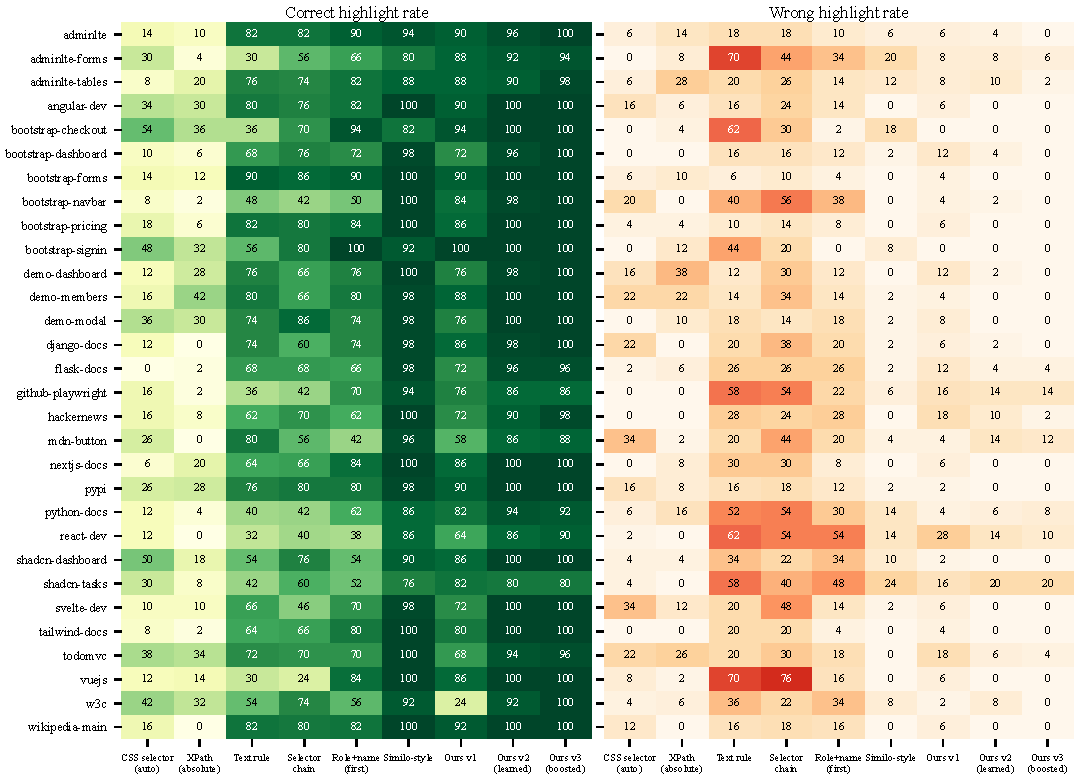
\includegraphics[width=\textwidth]{fig_perpage.pdf}
\caption{Per-page correct (left) and wrong (right) rates at composite redeploy $\rho{=}0.5$. Improvements are broad, not driven by one page; our fixture is not special. Wrong rates remain non-trivial on documentation pages with many near-identical links.}
\label{fig:perpage}
\end{figure*}

\subsection{Runtime cost}
\begin{figure*}[!t]
\centering
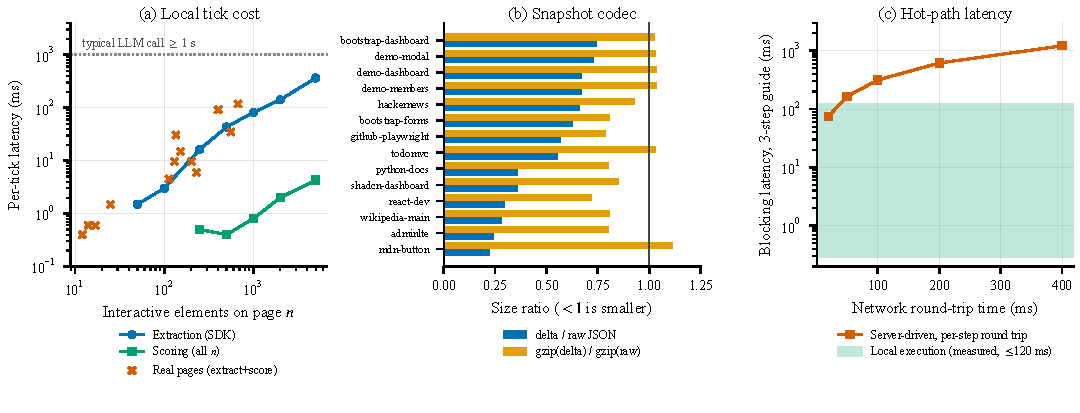
\includegraphics[width=\textwidth]{fig_efficiency.pdf}
\caption{(a)~Measured per-tick latency: extraction (DOM and style reads) dominates and grows with page size, scoring stays small; real pages are crosses. (b)~Snapshot-codec size relative to raw JSON, and after gzip. (c)~Blocking latency of a 3-step guide: server-driven is a \emph{model} (steps $\times$ (RTT $+$ 5\,ms measured server time)); the green band is the measured worst local tick.}
\label{fig:eff}
\end{figure*}
Fig.~\ref{fig:eff}(a) shows that a tick (extraction plus one score pass) takes a median of \tickMed\,ms across the \nTimed{} timed snapshots and at most \tickMax\,ms (the Wikipedia main page: 673 interactive elements, 250 kept). On synthetic pages extraction grows to \extOneK\,ms at 1{,}000 and \extFiveK\,ms at 5{,}000 interactive elements, while scoring all 5{,}000 takes \scoreFiveK\,ms; the cap of 250 therefore bounds scoring but not extraction. Even the worst measured tick is far below the typical latency of a model call.

The snapshot codec (Fig.~\ref{fig:eff}(b)) is lossless on all \nTimed{} timed snapshots (decode equals input) and shrinks raw JSON to a median of \codecMedian\% (range \codecBest--\codecWorst\%). After gzip, however, the median is \gzMedian\% and the worst case is \gzWorst\%, so the codec adds little once transport compression is on. We report this plainly; the codec's value is mostly in memory and parse cost, which we did not measure.

We walked the real invite flow through the real server (3 steps). The guidance path made one session-start request (5{,}174\,B) and three fire-and-forget checkpoints (532, 246 and 242\,B), with no blocking call on any step transition. A design that asks a server for every step needs at least one blocking round trip per step; Fig.~\ref{fig:eff}(c) models that cost. This is a model, not a measurement of a competing product.

\subsection{Engineering verification}
On the evaluated revision, all 23 shared and 36 server unit tests pass. The Playwright end-to-end suite (ten specification files covering duplicate buttons, forced remounts, portal modals, SPA routes, refresh-resume, placement, and the composer) was not re-run for this study, since it needs a bundled Chromium; the benchmark above used the system Chrome instead. Our fixture was written by us and may favour our design, which is why half of the corpus is public pages.

%% =====================================================================
\section{Discussion and Limitations}\label{sec:disc}
\textbf{What the results do and do not show.} They show that, under controlled structural drift, multi-signal matching beats the locator strategies that DAPs document, that our hand-weighted v1 was not competitive with a Similo-style matcher, that a linear learned ranker (v2) ties it, and that a boosted ranker (v3) is significantly better than it on held-out pages. They do not show that we beat the published state of the art, since our Similo-style arm is a simplified reimplementation and not the authors' code; v3 was not run in the leave-one-operator-out protocol, and and they do not show that our product beats Whatfix, WalkMe or any vendor: the baselines are our reimplementations of documented behaviour, vendors may ship undocumented repair, and the commercial platforms offer analytics, localisation and integrations that we do not.

\textbf{Scale and realism.} The corpus is 14 page states and the changes are synthetic; the strongest next validation is real before/after release pairs of the same site, and a run of the original Similo implementation. \textbf{Perturbations are synthetic.} Real redeploys differ from our operators, and the seeded composite weights are our choice. We therefore plot every intensity and operator separately (Figs.~\ref{fig:robust}, \ref{fig:robustwrong}). The Similo-style arm is our simplified reimplementation, not the authors' code; a run of the original is needed before any claim against Similo itself. v2 is trained and tested on synthetic perturbations of the same operator family (we mitigate with page-held-out and operator-held-out splits). Pages are static snapshots without scripts, so dynamic behaviour (late rendering, shadow DOM, cross-origin frames) is out of scope.

\textbf{Known weaknesses.} Exact name matching makes copy drift costly. The ordinal hint is positional. Section labels on real pages can be very long landmark texts. Extraction is capped at 250 elements, and its cost scales with page size. The language-model compiler is not quantitatively evaluated here: we have no live-API experiment, and the validation guard is covered only by unit tests.

\textbf{A defect found by the evaluation.} While counting requests we observed the SDK calling \texttt{GET /v1/onboarding} about eight times per second \emph{indefinitely} after a flow completes: the completion handler refreshes the discovery dock on every tick, and re-rendering the dock mutates the page and triggers the next tick. It does not affect the guidance-path numbers above (we excluded those requests), but it is a real inefficiency to fix.

\textbf{Statistical scope.} With 14 page states and a cluster bootstrap, intervals are honest but wide for page-sensitive arms (the criteria path especially). The margin-gate $\delta$ is cross-fitted, but both folds chose the same value from a coarse grid.

%% =====================================================================
\section{Conclusion}\label{sec:concl}
Guidance should not remember where a button was; it should work out which button is meant, and say so when it cannot. On \nPages{} page states and \nTrials{} resolutions, our first hand-weighted resolver beat documented DAP locator strategies but not a Similo-style weighted-similarity matcher. A linear learned ranker (v2) tied that matcher, and a boosted ranker (v3) on candidate-context features, tested on held-out pages, beat it significantly (\gbC\% against \simC\% correct; \gbW\% against \simW\% wrong). On the real Similo dataset the boosted ranker ties the authors' original code and the margin gate trades coverage for fewer wrong highlights; online feedback gave a negligible gain. Caveats remain: the synthetic-benchmark baseline is our reimplementation, the perturbations are synthetic, and v3 is not yet in the SDK. Longer feedback streams, a leave-one-operator-out run for v3, and in-browser latency measurements are the next experiments. Code, harness, and raw results are in the project repository \cite{project_repo}.

\bibliographystyle{IEEEtran}
\bibliography{ref}

\end{document}
